\documentclass[10pt,a4paper]{article}
\usepackage[margin=15mm,bottom=20mm]{geometry}
\usepackage{fontspec,xeCJK}
\setmainfont{Arial}
\setCJKmainfont{Microsoft YaHei}
\usepackage{graphicx,tikz,longtable,array,booktabs,amssymb,setspace,titlesec,fancyhdr,lastpage,hyperref}
\hypersetup{hidelinks,pdftitle={HollowHaven Technical Manual}}
\setstretch{1.65}
\setlength{\parindent}{0pt}\setlength{\parskip}{7pt}
\setlength{\emergencystretch}{3em}
\titleformat{\section}{\Large\bfseries}{\thesection.}{.5em}{}[\vspace{5pt}\titlerule]
\titleformat{\subsection}{\large\bfseries}{\thesubsection}{.5em}{}
\titlespacing*{\section}{0pt}{20pt}{12pt}
\titlespacing*{\subsection}{0pt}{16pt}{8pt}
\renewcommand{\arraystretch}{1.3}
\pagestyle{fancy}\fancyhf{}\renewcommand{\headrulewidth}{0pt}
\fancyfoot[C]{\fontsize{6}{8}\selectfont HollowHaven · \thepage\ / \pageref*{LastPage}}
\begin{document}
\thispagestyle{empty}
\begingroup
\definecolor{coverink}{HTML}{283540}
\definecolor{covergray}{HTML}{7C8791}
\setstretch{1}
\vspace*{12mm}
\noindent\hspace*{9mm}{\color{covergray}\fontsize{10}{14}\selectfont H O L L O W H A V E N}\par
\vspace*{64mm}
\noindent\hspace*{9mm}{\color{coverink}\fontsize{34}{42}\selectfont Technical Manual}\par
\vspace{8mm}
\noindent\hspace*{9mm}{\color{covergray}\fontsize{8}{12}\selectfont SYSTEM DOCUMENTATION}\par
\vfill
\noindent\hspace*{9mm}{\color{covergray}\fontsize{8}{12}\selectfont 2026.11\hspace{8mm}EDITION 01}\par
\vspace*{18mm}
\endgroup
\clearpage
\renewcommand{\contentsname}{Contents}
\begingroup\setstretch{1.05}\small\setcounter{tocdepth}{1}\tableofcontents\endgroup\clearpage
Wiring and Replication Guide · Version 5 November 2026. Signal assignments follow project\_config.h, project/README.md and CURRENT\_SETUP.md at Git revision e40f8b5. Board labels are based on the team's photographs. The 3D enclosure information remains as placeholders at the team's request; exact physical replication requires those details.


Revision: 2026-11-06. Reorganized into eight chapters; original cover and contents styling retained.
\section{Project introduction and technical objectives}
HollowHaven is a course prototype for integrating environmental monitoring, automatic gravity-fed watering and event-triggered audio recording in an artificial-hollow concept for Greater Gliders. The system combines ESP32 sensing and local control, a Node.js service and a browser dashboard. Blender models and a layered enclosure support physical integration. Cooling performance and long-term wildlife suitability still require experimental validation.

\clearpage
\section{System architecture and technology stack}

HollowHaven is a coursework functional prototype integrating sensing, automatic water delivery and event observation. It has not been validated as a long-term wildlife shelter. This manual explains the current implementation for builders and technical maintainers, alongside wiring, deployment and acceptance. Routine dashboard operation and maintenance belong in HollowHaven-User-Manual-English.pdf; the Chinese counterpart is HollowHaven-User-Manual-Chinese.pdf.

The implementation path is sensors $\rightarrow$ ESP32 acquisition and local control $\rightarrow$ TCP over a shared router network $\rightarrow$ Node.js validation and storage $\rightarrow$ browser monitoring. Valve decisions run on the ESP32. Computer disconnection interrupts reception but does not stop device-side control.

\begin{longtable}{p{49.333333333333336mm} p{49.333333333333336mm} p{49.333333333333336mm}}\toprule
\textbf{Layer} & \textbf{Current implementation} & \textbf{Responsibility}\\\midrule\endhead
Structure and water & Prototype body, elevated reservoir, servo valve and external wick & Gravity delivery and capillary spreading; wet layer separated from the cavity\\
Device & ESP32; ESP-IDF C firmware built with PlatformIO & I²C/ADC acquisition, moisture states, PWM, distance events and recordings\\
Local service & website/server.js; Node.js & Discovery, TCP reception, CSV/WAV storage, browser APIs and analysis requests\\
Browser & website/public/app.js, control-view.js and index.html & Live states, trends, maintenance indicators, archive and settings\\
Optional external service & Manually requested audio analysis & Candidate interpretations; no valve control or confirmed species identification\\
\bottomrule\end{longtable}

\clearpage
\section{Hardware design and implementation}

Prepare one classic ESP32-WROOM-32 development board and the photographed expansion baseboard; one SHT3x module, one VL53L0X module and one SEN0487 microphone; two capacitive moisture modules; one analogue light module, one water-level module and one MG90S servo. Also prepare wicking material, a reservoir, tubing, a valve mechanism compatible with the servo, jumper wires, a USB data cable, a power bank, a multimeter, a computer and mounting hardware.

Exact purchasing references, connector dimensions and valve model: [TO BE COMPLETED]. Confirm that the modules support 3.3 V power and signals. A bare sensor chip is not a direct replacement for a breakout module with its supporting circuitry.

Tools: multimeter, insulated tools, small screwdriver and cable ties. Assemble and test the electronics and software on the bench before fitting the enclosure. Verify the dry assembly before introducing water.


Orient the board with its USB connector at the bottom and its metal shield towards the top. Labels visible on the left include VP, VN, D34, D35, D32, D33, D25, D26, D27, D14, D12 and D13. D22 and D21 are visible on the right. On this board, D-number labels refer to the corresponding GPIO number. VP is GPIO36 and VN is GPIO39. VP is not a positive power terminal.

These are GPIO numbers, not the computer's COM port. The COM identifier can change with the computer or USB port and must be identified before flashing. The photographs establish labels and some connector locations, but do not reveal every obscured wire endpoint. The diagram represents the connections required by the firmware.

Some D21/D22 connectors may be duplicate breakouts; verify continuity with power disconnected. The baseboard schematic is unavailable, so do not assume the inner-to-outer S/V/G order. Identify ground, supply and signal before attaching modules.


The embedded diagram shows coloured signal paths. VCC/GND labels beneath each module identify additional required power connections; identically named networks connect together. Colours are illustrative and do not identify the actual jumper wires. Verify terminal labels at both ends of every connection.

\par\vspace{2mm}\noindent\begin{minipage}{\linewidth}\centering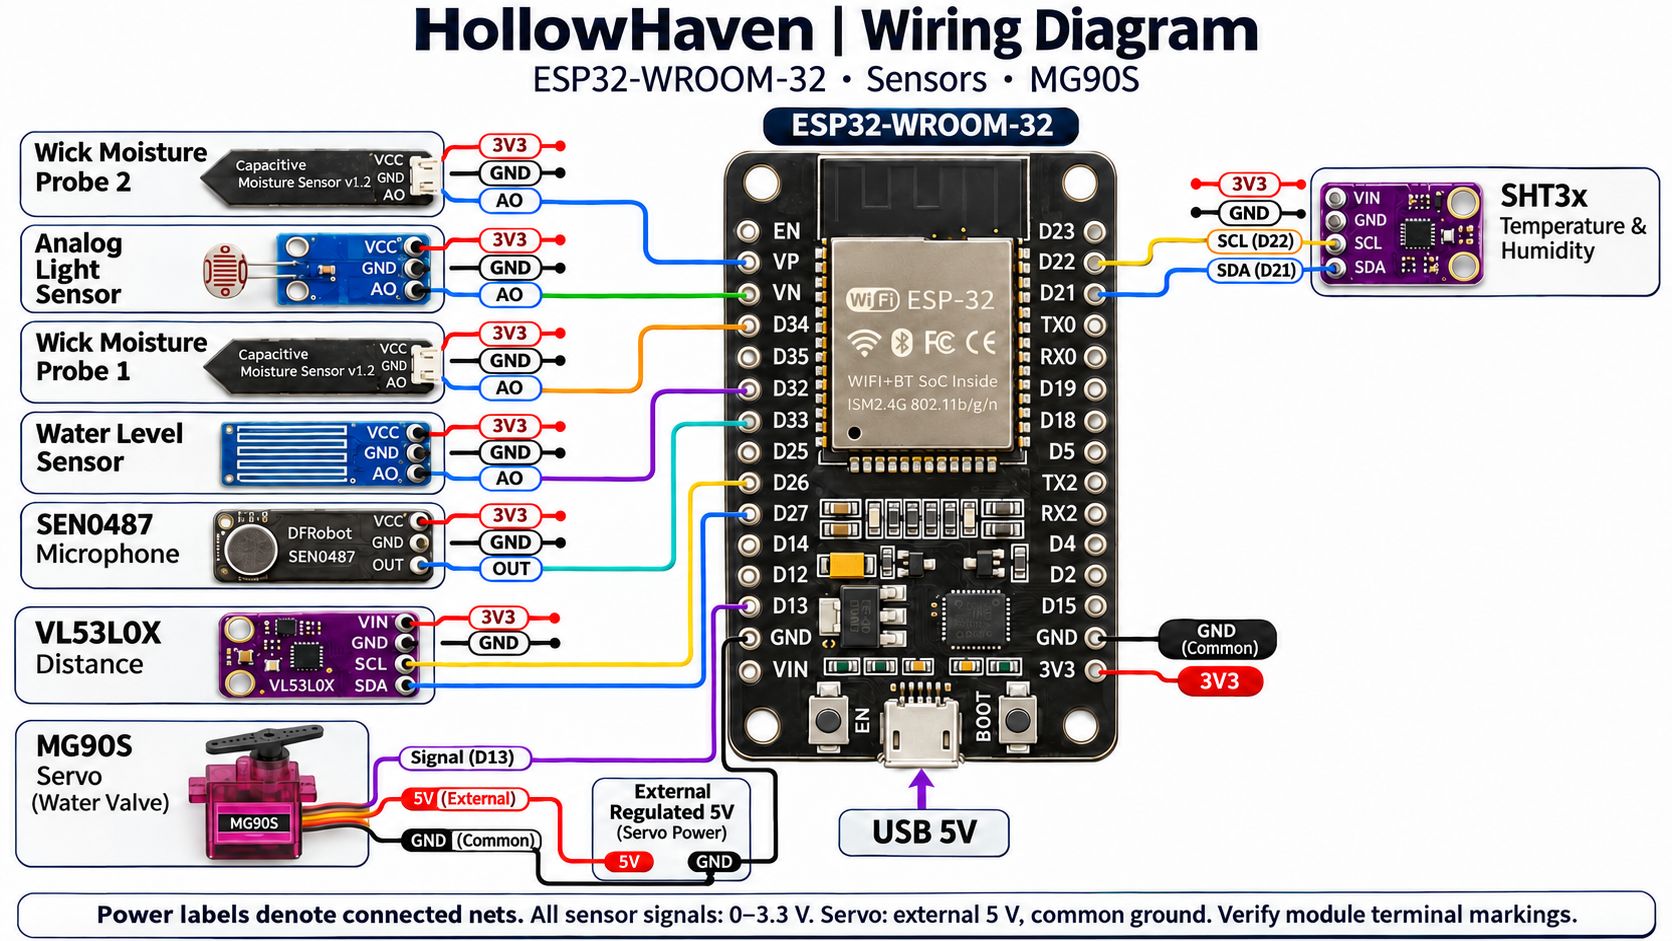
\includegraphics[width=\linewidth,keepaspectratio]{wiring-realistic.png}\par{\small Wiring diagram}\end{minipage}\par\vspace{2mm}
Power the ESP32 development board through its USB connector from a standard regulated 5 V USB external supply such as a power bank. Use a computer USB data cable for flashing. Compatible sensors use 3.3 V; the servo uses 5 V with common ground, as shown below.

\begin{longtable}{p{49.333333333333336mm} p{49.333333333333336mm} p{49.333333333333336mm}}\toprule
\textbf{Module terminal} & \textbf{ESP32 terminal} & \textbf{Notes}\\\midrule\endhead
SHT3x SDA / SCL & D21 / D22 & First I²C bus; do not interchange the two wires\\
SHT3x VCC / GND & 3V3 / GND & Use a 3.3 V-compatible module\\
Moisture 1 AO / VCC / GND & D34 / 3V3 / GND & First wicking-material location\\
Moisture 2 AO / VCC / GND & VP (GPIO36) / 3V3 / GND & Neither D35 nor VN\\
Light AO / VCC / GND & VN (GPIO39) / 3V3 / GND & Use analogue AO, not digital DO\\
Water level AO / VCC / GND & D32 / 3V3 / GND & 3.3 V-compatible module; reading is not continuous volume\\
SEN0487 A / VCC / GND & D33 / 3V3 / GND & Analogue microphone output\\
VL53L0X SDA / SCL & D27 / D26 & Separate second I²C bus\\
VL53L0X VIN / GND & 3V3 / GND & Compatible breakout; leave XSHUT and GPIO1 unused\\
MG90S signal & D13 & PWM; verify the manufacturer's terminal identification\\
MG90S positive supply & Separate regulated 5 V branch & Do not connect to ESP32 3V3\\
MG90S supply negative & Common GND & Connect to ESP32 ground\\
\bottomrule\end{longtable}
DS18B20 is not connected and its D4 function is disabled. TX0/RX0 are not used for these sensors. All analogue signals must remain within 0–3.3 V. A module with a 5 V output requires an appropriate level interface before connection.


SHT3x measures cavity temperature and humidity on one I²C bus; VL53L0X measures distance on another. Light, water level, both wick probes and the microphone use ADC1, avoiding the classic ESP32 Wi-Fi/ADC2 conflict. Raw ADC counts are not lux, millilitres, moisture percentage or sound pressure level. External DS18B20 measurement is disabled.

The prototype uses an elevated reservoir, gravity-fed tubing and a servo-operated valve to supply an external wicking layer. Capillary action distributes water; evaporation may reduce heat transfer into the cavity under suitable humidity and airflow. Bark-like covering supports shading and ecological context, but appearance cannot establish insulation or cooling performance. Rain collection, where retained, is a design intention until collection efficiency, filtration and overflow are measured. Exact mechanical dimensions await team measurements.

Valid light and temperature initiate watering; a minimum open duration and periodic temperature decisions maintain the cycle. Two wick probes check water arrival at separate locations, raising a possible supply fault when dryness persists after full opening. Water level independently requests refilling. Commanded position, material wetting and measured flow are different evidence: the system has neither a flow meter nor mechanical position feedback. Thresholds appear in the control section below.


\clearpage
\section{Software design and implementation}

presence\_sensor.c and shared/presence.h confirm suspected entry using consecutive distance samples and separate entry/exit thresholds. Entry requests about 30 seconds of recording; continuous occupancy does not repeatedly retrigger it. analog.c acquires microphone PCM and metrics, while audio\_record.c manages limited Flash buffers and delivery. Distance and audio do not establish species identity.

The computer discovers the device through UDP 9002, then receives telemetry on TCP 9000 and audio on TCP 9001. Telemetry uses a version header and CSV rows with boot identity, sequence, uptime, validity and control states; the computer adds reception time. Audio carries metadata, PCM and CRC32; the receiver validates and writes WAV before acknowledgement. CRC checks transport integrity, not gap-free acquisition. Flash storage is limited: offline recordings may be overwritten, and complete offline telemetry history is not backfilled.


Step-by-step browser operation belongs in the user manual. This section retains functional scope and code responsibilities. The accompanying user manuals now include screenshot-based instructions for live monitoring, trends, CSV export, recordings, WAV import and settings.

\begin{longtable}{p{77.0mm} p{77.0mm}}\toprule
\textbf{Function} & \textbf{Implementation and boundaries}\\\midrule\endhead
Live monitoring and alerts & Temperature, humidity, distance, audio, valve, wick states and maintenance indicators; invalid or stale data do not establish normal conditions\\
Trends and export & Up to 900 recent samples retained for display; CSV persists on disk and export corresponds to the current server session\\
Recording archive & Up to 250 recent WAV files displayed, with search, waveform, playback, download and WAV import; display limit is not deletion policy\\
Audio analysis & Explicit user request sends a selected file through Node.js to the configured provider; results remain unverified candidates\\
Settings and language & Device address, analysis provider and options; API key held only in process memory and re-entered after restart\\
\bottomrule\end{longtable}
website/protocol.js parses telemetry and validates audio. server.js handles connections, persistence and APIs. public/app.js manages browser interactions, and public/control-view.js renders valve and maintenance states. The dashboard has no manual valve switch. Closing the browser or pausing reception does not change firmware thresholds. Threshold changes require rebuilding and reflashing, with corresponding documentation and acceptance updates.

Telemetry is stored in website/data/session\_*.csv, audio in website/recordings/, results in website/data/results.json and non-secret settings in settings.json. The browser accesses Node.js at \url{http://127.0.0.1:8766} rather than reading sensors directly. Diagnose acquisition, transport, server reception and browser rendering as separate stages.


Valid light ADC below 500 and valid temperature above 30°C request opening. Once the commanded fully open position is reached, hold at least 60 seconds and check once per minute. Close only below 26°C; otherwise remain open. Later light changes do not end the cycle. Invalid temperature prolongs opening. Low water warns only and does not inhibit opening. This corrects the older manual's statement that temperature does not participate in control.

Servo output is 50 Hz: 1200 μs open and 2500 μs closed, changing by 10 μs every 100 ms. Calibrate travel against the actual mechanism and avoid forcing mechanical stops. Displayed position is commanded position, without mechanical feedback.

For both moisture channels, ADC below 2000 means wet and at least 2300 means dry. Intermediate readings retain the previous state; an initial intermediate or invalid reading is unknown. Either point remaining dry after at least 60 seconds fully open triggers possible blockage. Record dry, wet and intermediate readings before adjusting thresholds.

Water ADC below 50 requests refilling; the “below 50 ml” label is not a volume measurement. Light is raw ADC, not lux: verify direction with actual shading and illumination. Three consecutive distance readings at or below 189 mm trigger entry; five at or above 220 mm clear occupancy, with approximately 100 ms sampling. Remeasure empty-cavity distance in the completed enclosure. Entry triggers approximately 30 seconds of audio.


\clearpage
\section{3D modelling and mechanical design}

Full-size design benchmark: floor 250 × 300 mm, height 550 mm and entrance diameter 85 mm. Source: Victorian Government wildlife rehabilitation guidelines, Chapter 9, page 385, \url{https://www.wildlife.vic.gov.au/}\_\_data/assets/pdf\_file/0021/671250/Part-B-Mammals-Chapter-9.pdf . These rehabilitation-context dimensions are the project's adopted benchmark; actual prototype measurements remain separate and field suitability is not established.

The following fields are intentionally blank. They are not manufacturing specifications until completed. Use millimetres throughout.

\begin{longtable}{p{77.0mm} p{77.0mm}}\toprule
\textbf{Item} & \textbf{Information required}\\\midrule\endhead
Overall dimensions & Height [TBD] × width [TBD] × depth [TBD]\\
Body and lid & Material [TBD]; wall thickness [TBD]; STL/STEP files [TO BE PROVIDED]\\
Entrance & Diameter [TBD]; height above base [TBD]; orientation [TBD]\\
Resting cavity & Internal diameter or width/depth [TBD]; usable height [TBD]\\
Electronics bay and service opening & Dimensions, water separation and access method [TBD]\\
Mounting & Hole sizes/spacing, fasteners and tree attachment method [TBD]\\
Reservoir and water path & Capacity, position, tube diameter, valve, outlet and leak prevention [TBD]\\
Wicking layer & Material, dimensions, routing and separation from resting space [TBD]\\
Servo bracket & Mounting centres, linkage, travel limits and valve coupling [TBD]\\
Sensor placement & Each sensor's distance from entrance, base and wicking layer [TBD]\\
Bark finish & Actual material, attachment and surface treatment [TBD]\\
Printing settings & Process, layer height, infill, supports and orientation [TBD]\\
\bottomrule\end{longtable}
Suggested assembly order: fabricate and deburr the enclosure; trial-fit the electronics bay and reservoir; dry-fit the valve, servo bracket and tubes; position the wicking layer and two moisture points; install temperature/humidity, distance and microphone modules; secure the harness; verify the electronics; finally introduce water. This is assembly guidance, not a claim that the missing design has been finalised.

The temperature/humidity sensor should observe cavity air rather than touch wet cloth. Keep wiring and enclosure surfaces out of the distance sensor's field of view. Protect the microphone from water and separate it from servo vibration where practical. The moisture sensors must observe different locations. Record final positions in the manufacturing drawings rather than relying only on photographs.

\subsection{Three-layer enclosure}
From inside to outside, the prototype comprises a perforated ventilation layer, a wicking layer and an outer bark layer. Multiple openings in the inner layer provide paths for air circulation. The middle layer uses horticultural capillary matting to absorb and spread water. The outer bark provides a tree-like finish. Capillary transport is passive and does not require an additional pump.

The matting is intended to reduce concentration of water at the lowest point and help maintain wetting when the enclosure is tilted. Actual uniformity depends on inclination, continuous material contact, supply rate and evaporation. Maintain contact across the matting, avoid folds obstructing ventilation holes, and route moisture and drainage away from the resting cavity and electronics.

Test upright and at the intended inclination, recording wetting response at both probes and inspecting upper, lower and circumferential areas. Two readings support inspection but do not establish whole-surface uniformity. Hole diameter, count, spacing and layer thickness remain to be supplied.

\par\vspace{2mm}\noindent\begin{minipage}{\linewidth}
\begin{minipage}[t]{0.47\linewidth}\centering\vspace{0pt}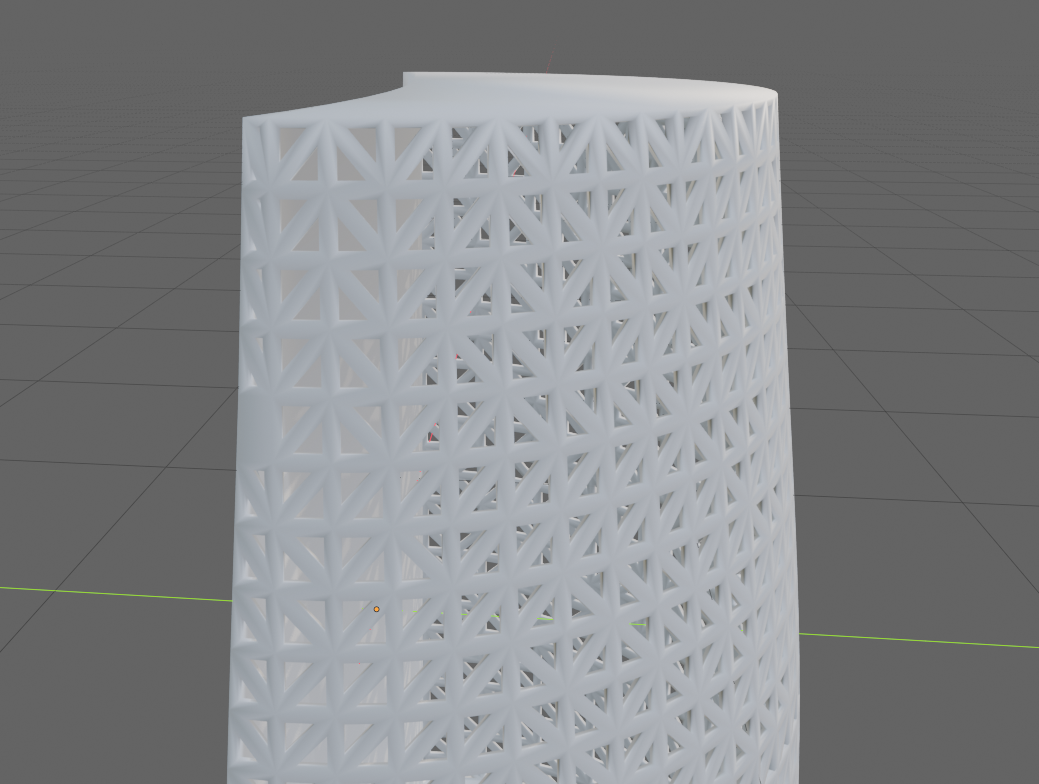
\includegraphics[width=\linewidth,height=46mm,keepaspectratio]{images/M1.png}\par\vspace{2mm}{\setstretch{1.1}\footnotesize Figure M1 Ventilation-layer 3D detail: curved lattice and triangular openings. Dimensions are not shown.\par}\end{minipage}\hfill \begin{minipage}[t]{0.47\linewidth}\centering\vspace{0pt}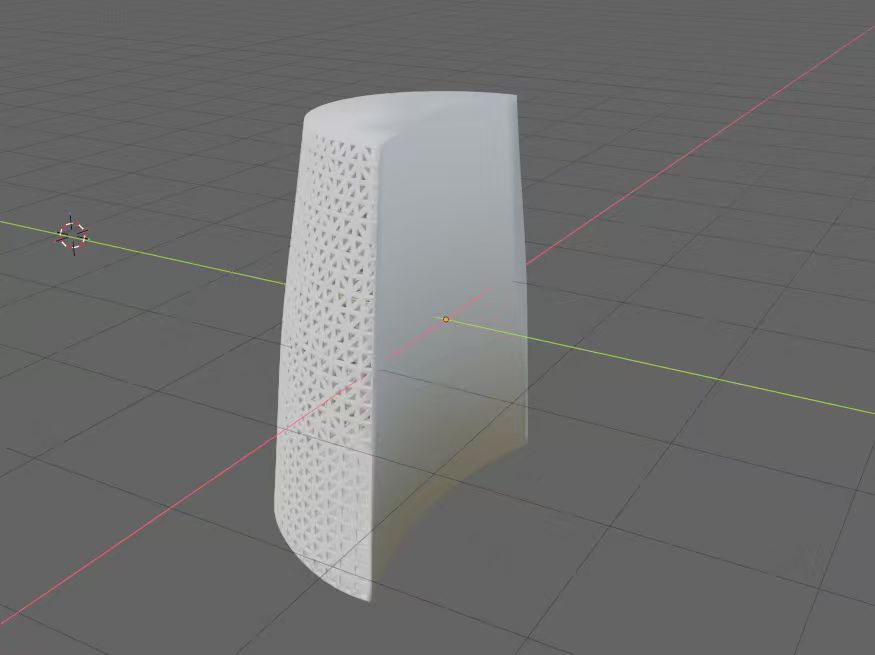
\includegraphics[width=\linewidth,height=46mm,keepaspectratio]{images/M2.jpg}\par\vspace{2mm}{\setstretch{1.1}\footnotesize Figure M2 Overall 3D view of the curved ventilation shell, perforated area and continuous edges.\par}\end{minipage}\par\vspace{3mm}
\begin{minipage}[t]{0.47\linewidth}\centering\vspace{0pt}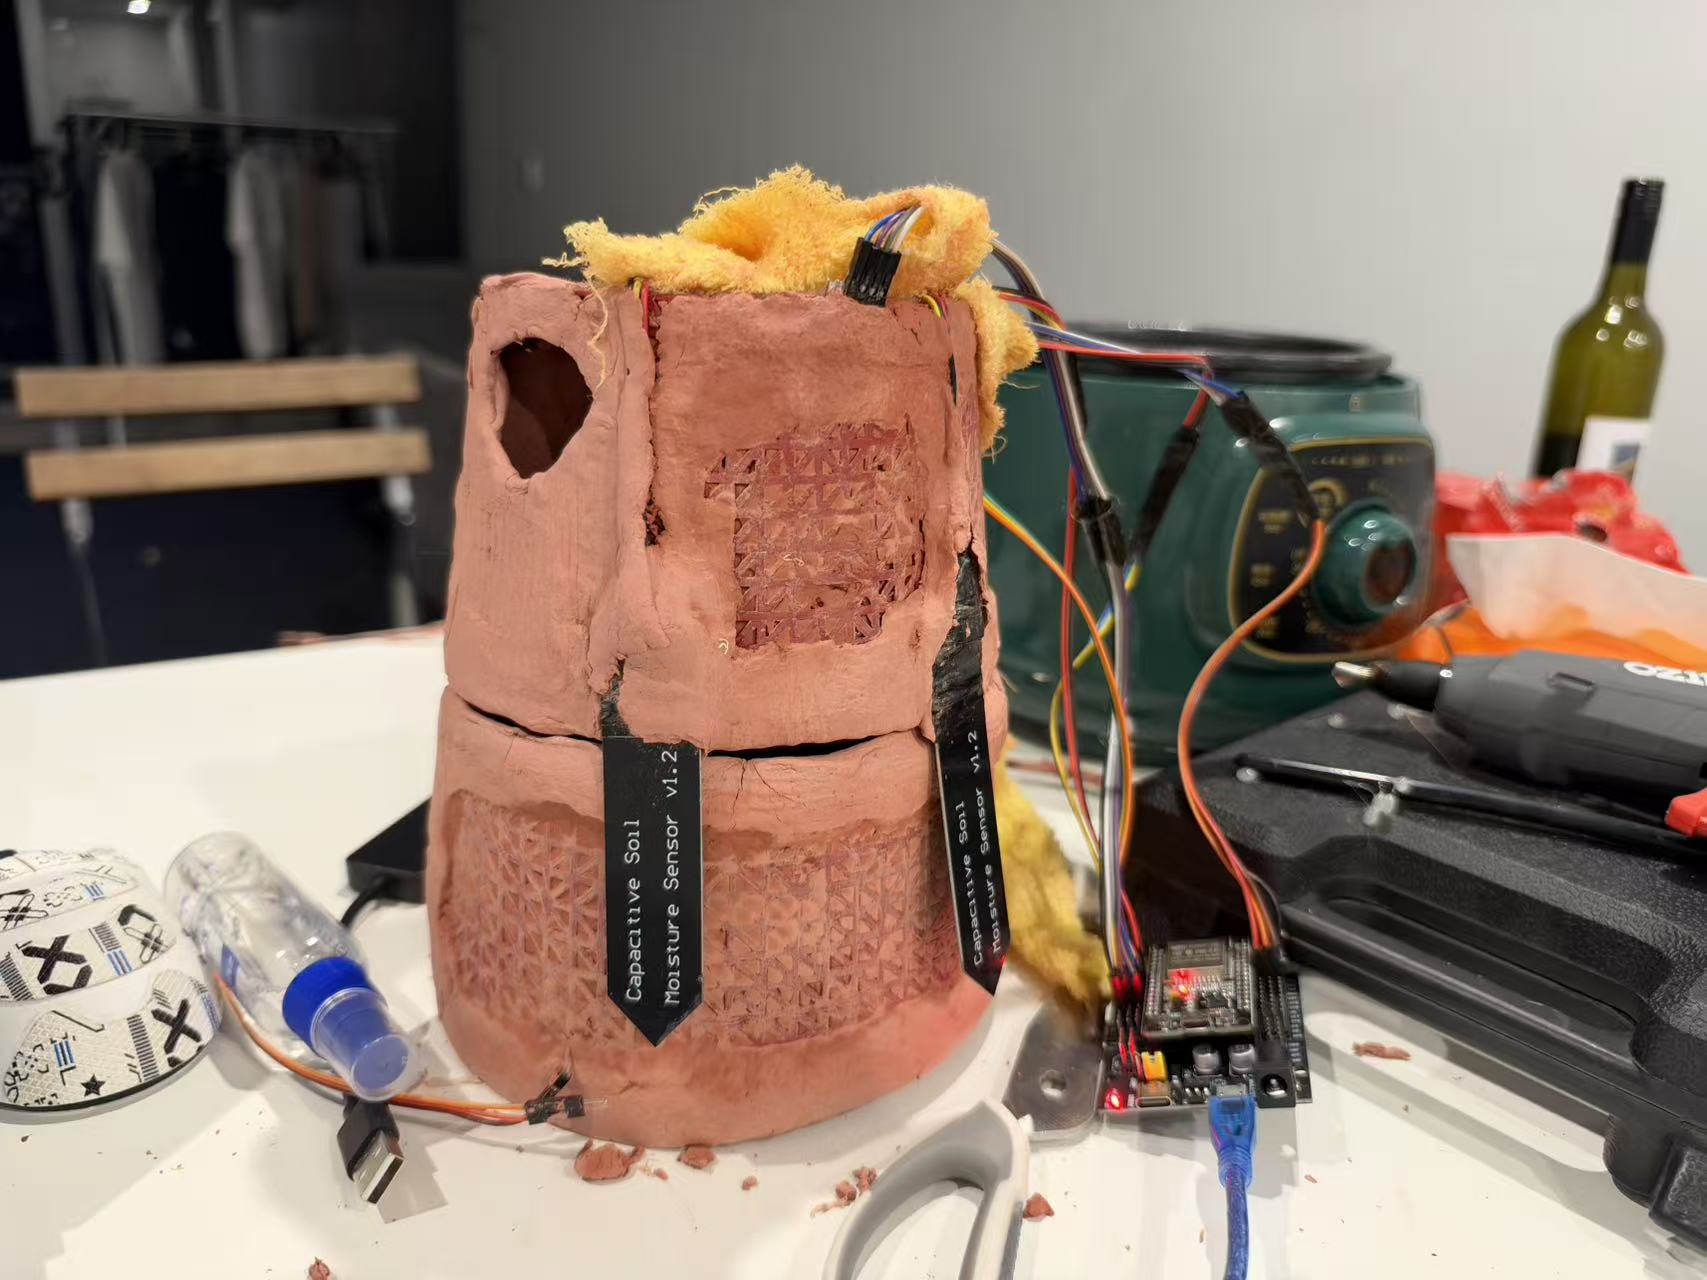
\includegraphics[width=\linewidth,height=46mm,keepaspectratio]{images/M3.jpg}\par\vspace{2mm}{\setstretch{1.1}\footnotesize Figure M3 Assembly stage: entrance, ventilation lattice, two capacitive probes and external ESP32.\par}\end{minipage}\hfill \begin{minipage}[t]{0.47\linewidth}\centering\vspace{0pt}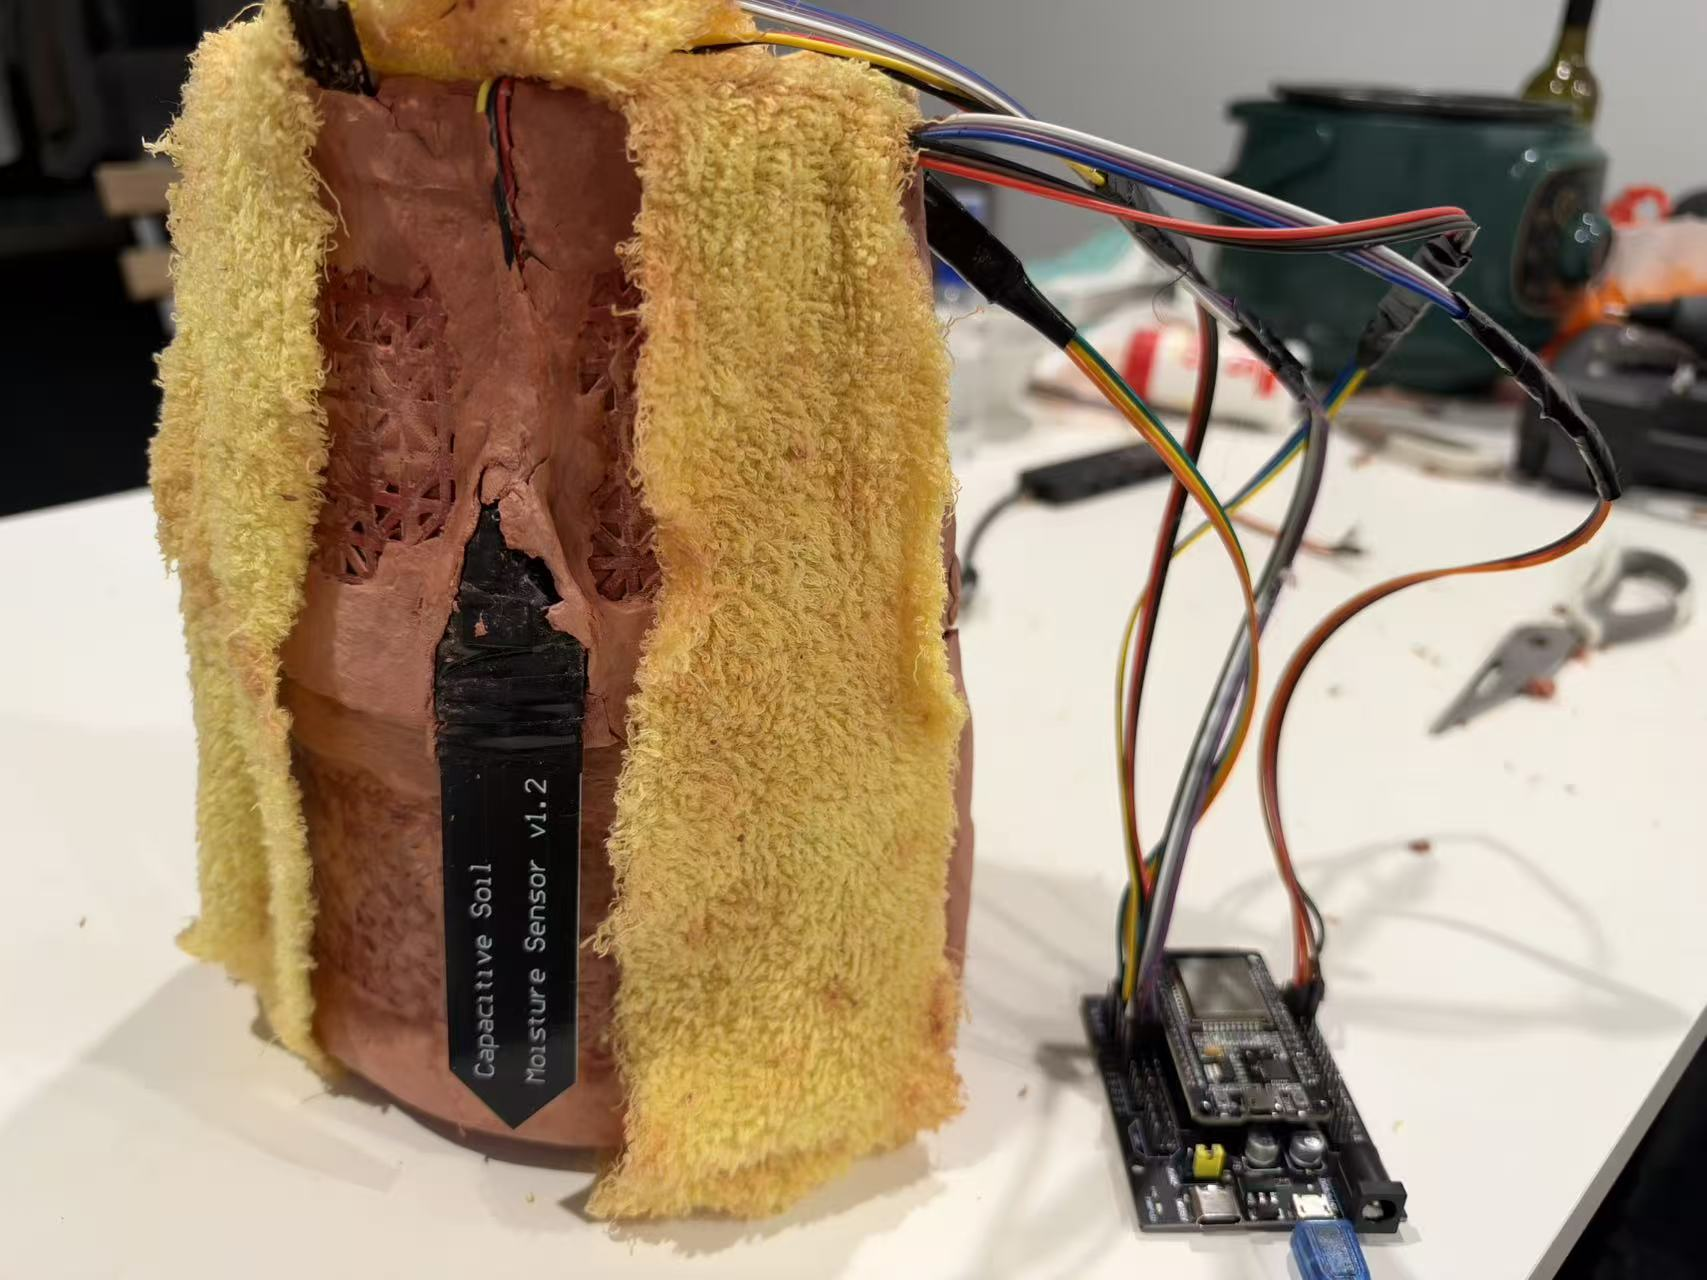
\includegraphics[width=\linewidth,height=46mm,keepaspectratio]{images/M4.jpg}\par\vspace{2mm}{\setstretch{1.1}\footnotesize Figure M4 Wicking-layer assembly: yellow horticultural capillary matting laid along the body beside moisture-monitoring locations.\par}\end{minipage}
\end{minipage}\par\vspace{2mm}
\par\vspace{2mm}\noindent\begin{minipage}{\linewidth}\centering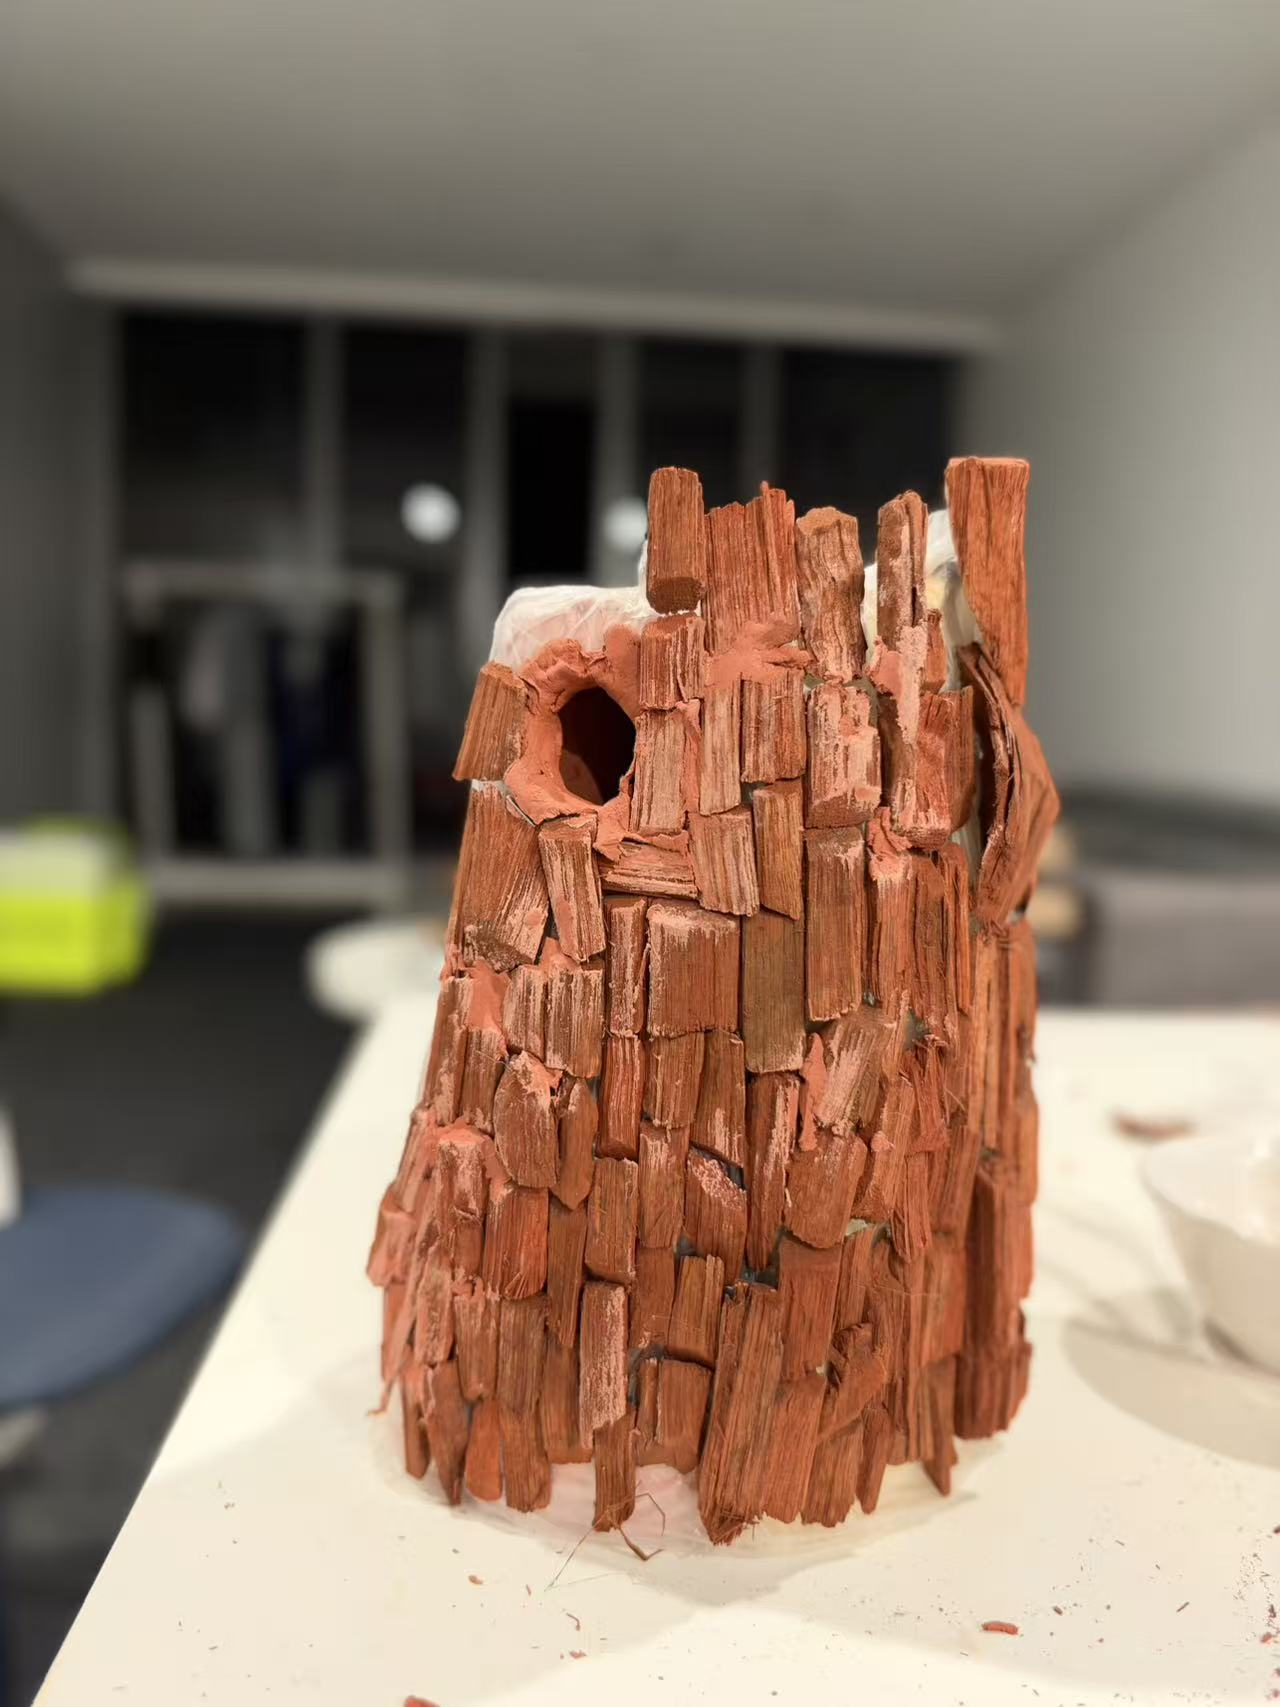
\includegraphics[width=0.40\linewidth,height=55mm,keepaspectratio]{images/M5.jpg}\par{\small Figure M5 Outer bark finish: overlapping bark pieces with the entrance retained.}\end{minipage}\par\vspace{2mm}
These team-supplied design views and photographs document different assembly stages. They show structure and placement; prototype dimensions, material thickness and attachment details still require measurement.


\clearpage
\section{Enclosure fabrication and system assembly}
Complete the electronics and software on the bench before installing them in the enclosure. Prepare and deburr the shell, trial-fit the tank and electronics, and dry-fit the valve, servo bracket and tubing. Fit continuous capillary matting and place the two moisture probes at different locations. Install the air-temperature sensor, distance sensor and microphone without obstructing the sensing area. Secure wiring, apply the bark covering while retaining the entrance and service access, and only then add water and check for leakage. Record the actual materials, dimensions and fasteners; the photographs do not supply manufacturing tolerances.

Test wetting in both upright and expected tilted orientations. Keep drainage and the wet layer away from electronics and the resting space. Two wetness readings do not establish uniform wetting over the whole enclosure.

\clearpage
\section{System testing and result recording}

\begin{enumerate}
\item Disconnect all power. Check ground continuity, signal endpoints and shorts. Temporarily disconnect the servo linkage from the valve.
\item Power only the ESP32. Check serial startup and the 3V3 rail, then disconnect power before adding sensors. Power off before every wiring change.
\item Connect SHT3x first and confirm valid temperature/humidity. Add VL53L0X and check distance changes with a test object.
\item Add analogue modules individually. Record dry/wet, shaded/lit, water-level and sound responses. Floating readings from an unplugged input do not demonstrate correct hardware operation.
\item Connect the separate 5 V servo supply with common ground. Test unloaded direction and approximately 13-second full travel before attaching the linkage. Check for binding.
\item Add water and verify that both monitored wicking locations actually become wet. Inspect the electronics bay and resting space for leakage. An open display does not prove water flow.
\item Save a CSV and WAV, restart the system and confirm reconnection. Record supply details, firmware revision, sensor placement and calibration values.
\end{enumerate}
\subsection{Evidence and outstanding measurements}
This revision does not report a new physical experiment. Source code supports implementation descriptions and photographs support assembly relationships. Record firmware version, sensor positions, raw readings, expected and observed behaviour, timestamps and output files for each test. Cooling claims require comparable watered and unwatered conditions, ambient temperature and humidity records, repeated measurements and stated sensor uncertainty. Quantitative thermal results and complete manufacturing dimensions remain to be supplied.

\clearpage
\section{Replication advice and future improvements}

Clone the repository with git clone \url{https://github.com/SMGG2302/comp-5047.git} . This guide corresponds to e40f8b5; use git checkout e40f8b5 to reproduce that revision. For a newer revision, recheck project\_config.h and CURRENT\_SETUP.md.

Install Node.js 18 or later and PlatformIO. The firmware directory is project/firmware. Copy wifi\_credentials.example.h to wifi\_credentials.h and enter the local 2.4 GHz router credentials. Do not commit real credentials.

In project/firmware, run pio run, then pio device list. Flash with pio run -t upload --upload-port COMx and monitor with pio device monitor -p COMx -b 115200. Replace COMx with the identifier reported by the operating system. The first build downloads the toolchain. Retain partitions.csv to preserve the audio-cache partition layout.

If Windows builds fail because of non-ASCII paths, review build-ascii.ps1 and update its machine-specific build and PlatformIO paths before using it. Other computers may not have those directories.

In website, run node server.js and open \url{http://127.0.0.1:8766.} Connect the computer and ESP32 to the same router without client isolation. Select auto discovery or enter the IP printed by the serial monitor. Discovery uses UDP 9002, telemetry TCP 9000 and audio TCP 9001. Avoid running a competing receiver at the same time.


\begin{longtable}{p{77.0mm} p{77.0mm}}\toprule
\textbf{Symptom} & \textbf{Check first}\\\midrule\endhead
No COM device & Data-capable USB cable, connectors, driver and port identification\\
Reset during servo motion & Supply branch, common ground, voltage drop and mechanical stall\\
Incorrect second moisture channel & Wrong D35/VN connection; correct input is VP/GPIO36\\
Invalid temperature/humidity or distance & Mixed I²C buses, swapped SDA/SCL, power and ground\\
Fixed extreme or drifting analogue readings & Signal voltage, AO rather than DO, loose wire or absent module\\
Device missing from dashboard & Same LAN, client isolation, firewall, serial IP and other receivers\\
Material remains dry after opening & Empty reservoir, blockage, valve not physically open, material placement/contact\\
\bottomrule\end{longtable}

Supply this manual, editable SVG diagram, revision-pinned source, complete purchasing BOM, CAD and dimensioned drawings, print settings, assembly photographs, calibration records and power-up acceptance records. The next builder must supply their own Wi-Fi credentials and AI key.

The wiring and electrical/software replication steps are supplied here. CAD and dimensions remain to be completed. Completing the mechanical specifications and passing staged acceptance are necessary for a complete physical replication handover.


UMass Amherst, Subirrigation Systems, uses capillary mat for horticultural material that transfers water through capillary action. This terminology does not establish the prototype material composition or specification. Source: \url{https://www.umass.edu/agriculture-food-environment/greenhouse-floriculture/fact-sheets/subirrigation-systems}


\end{document}